\subsection*{A Generic BVP}

%% \begin{frame}
%%   %\frametitle{}
%%   \begin{columns}[t]
%%     \column{.5\textwidth}
%%     \begin{block}{}%A general class of PDE}      %find $u(\bv{x},t)$ such that
%%       For this talk we will assume there is a
%%       mathematical model (PDE) to be solved in an engineering analysis:
%%       \begin{eqnarray}
%% 	\label{eqn:general_pde}
%% 	\nonumber
%% 	%\frac{\partial u}{\partial t} +
%% 	\R( u ) & = & 0 \;\;\;\;\; \in \Omega
%% 	\\
%% 	\nonumber
%% 	u & = & u_D \;\; \in \partial \Omega_D
%% 	\\
%% 	\nonumber
%% 	\nabla u \cdot n & = & u_N \;\; \in \partial \Omega_N
%% %% 	\\
%% %% 	\nonumber
%% %% 	u(\bv{x}, 0) & = & u_0(\bv{x})
%%       \end{eqnarray}
%%     \end{block}
%%     %\pause
%%     \column{.5\textwidth}
%%     %\begin{block}{}
%%       \begin{center}
%% 	%\fbox{
%% 	%\includegraphics[width=2in,angle=-90]{domain}
%%         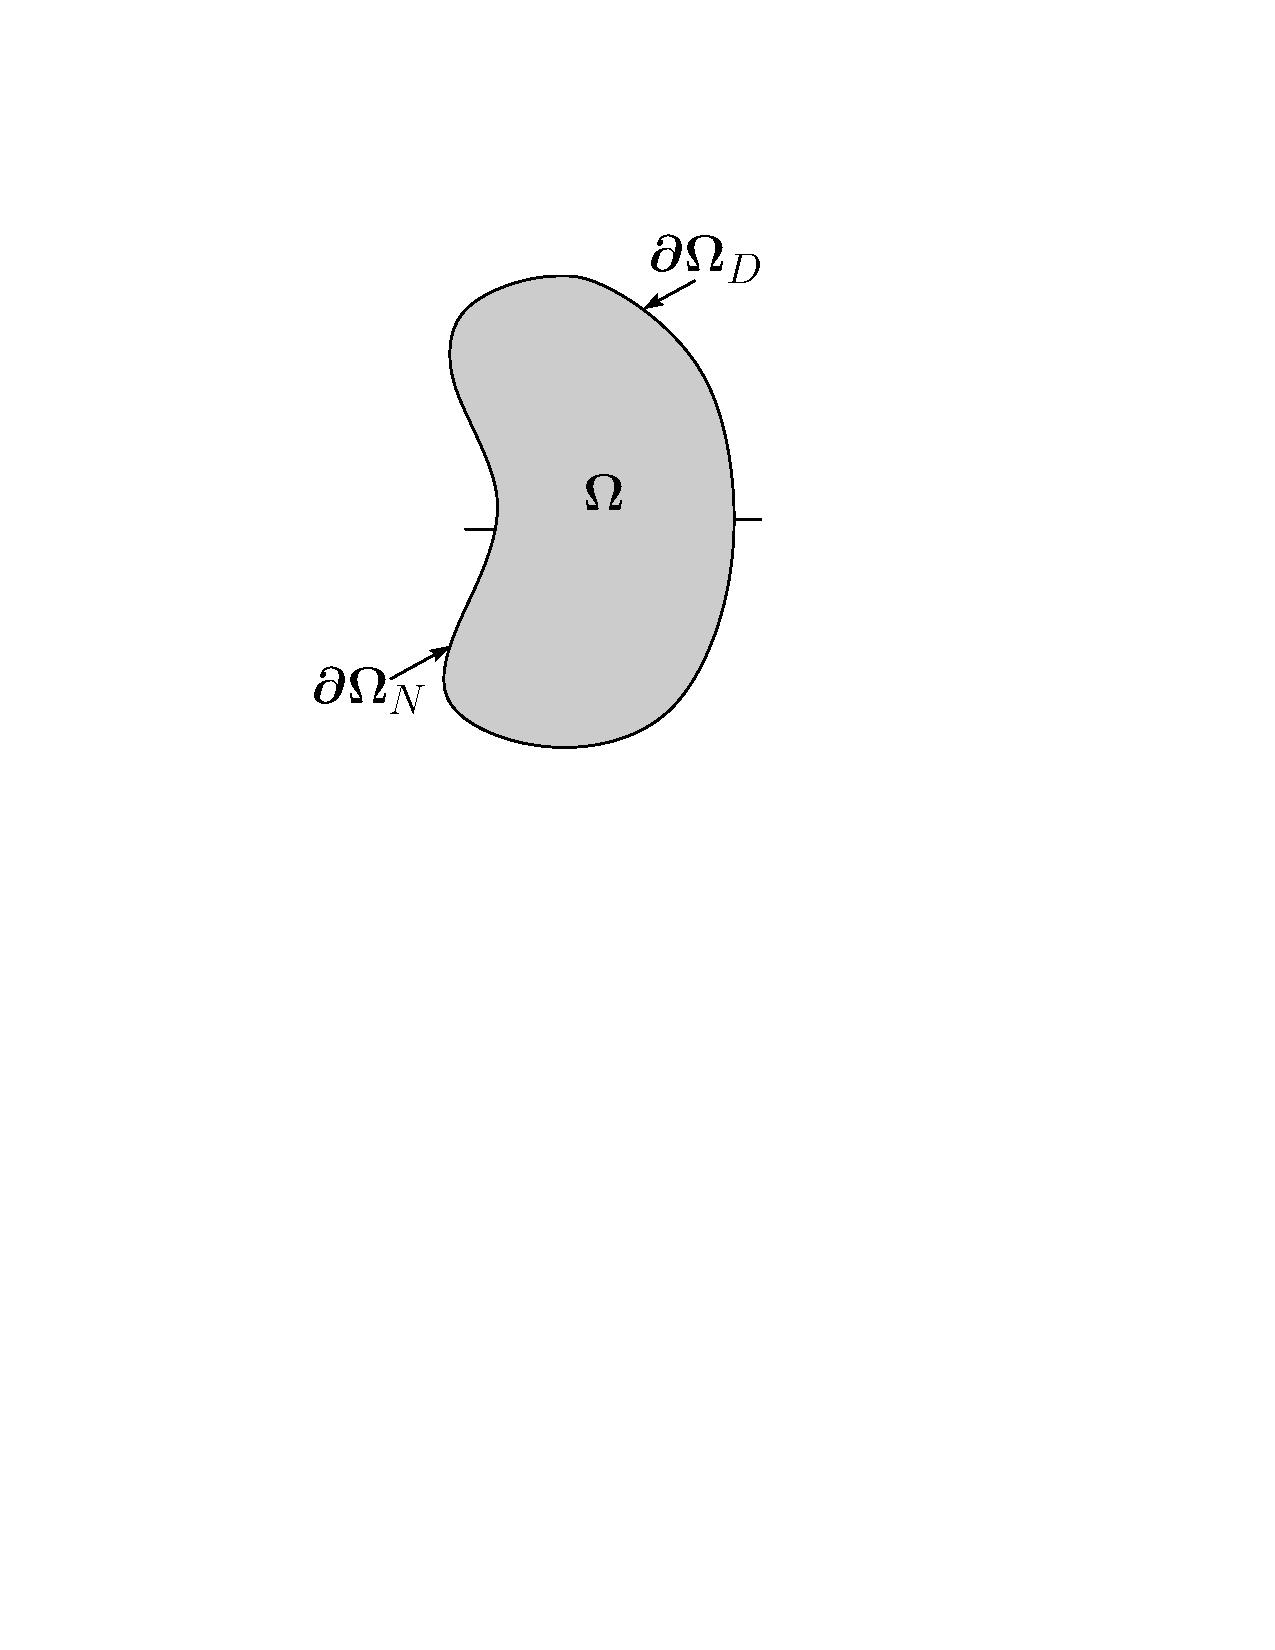
\includegraphics[viewport=140 420 400 685,clip=true,width=2in]{domain2/domain2_input}
%% 	%}
%%       \end{center}
%%     %\end{block}
%%   \end{columns}
%% %%  \begin{itemize}
%% %%    \item $\mathcal{N}( u )$ is a nonlinear operator which depends on the unknown
%% %%      $u$ and its spatial gradients%, $\bv{f}$ is a forcing function
%% %%    % \item With slight modifications, a wide range of physically interesting problems fall into this class
%% %%    \item Use generic numerical methods to treat many problems in the same framework
%% %%  \end{itemize}
%% \end{frame}



% The ``Generic BVP'' slide has been slightly revamped for notational consistency
\begin{frame}
  %\frametitle{A Generic BVP}
  \begin{columns}[t]
    \column{.5\textwidth}
    \begin{block}{A general class of PDE}      %find $u(\bv{x},t)$ such that
      \begin{itemize}
      \item We assume there is a Boundary Value Problem
      of the form to be approximated in an FE function space
      \end{itemize}
      \vspace{-.1in}
      \begin{eqnarray}
	\label{eqn:general_pde}
	\nonumber
	M \frac{\partial u}{\partial t} & = & F( u ) \;\;\;\; \in \Omega
        \\
	\nonumber
	G( u ) & = & 0 \;\;\;\;\;\;\;\;\; \in \Omega
	\\
	\nonumber
	u & = & u_D \;\;\;\;\;\;\; \in \partial \Omega_D
	\\
	\nonumber
	N(u) & = & 0 \;\;\;\;\;\;\;\;\; \in \partial \Omega_N
 	\\
 	\nonumber
 	u(\bv{x}, 0) & = & u_0(\bv{x})
      \end{eqnarray}
    \end{block}
    %\pause
    \column{.5\textwidth}
      \begin{center}
	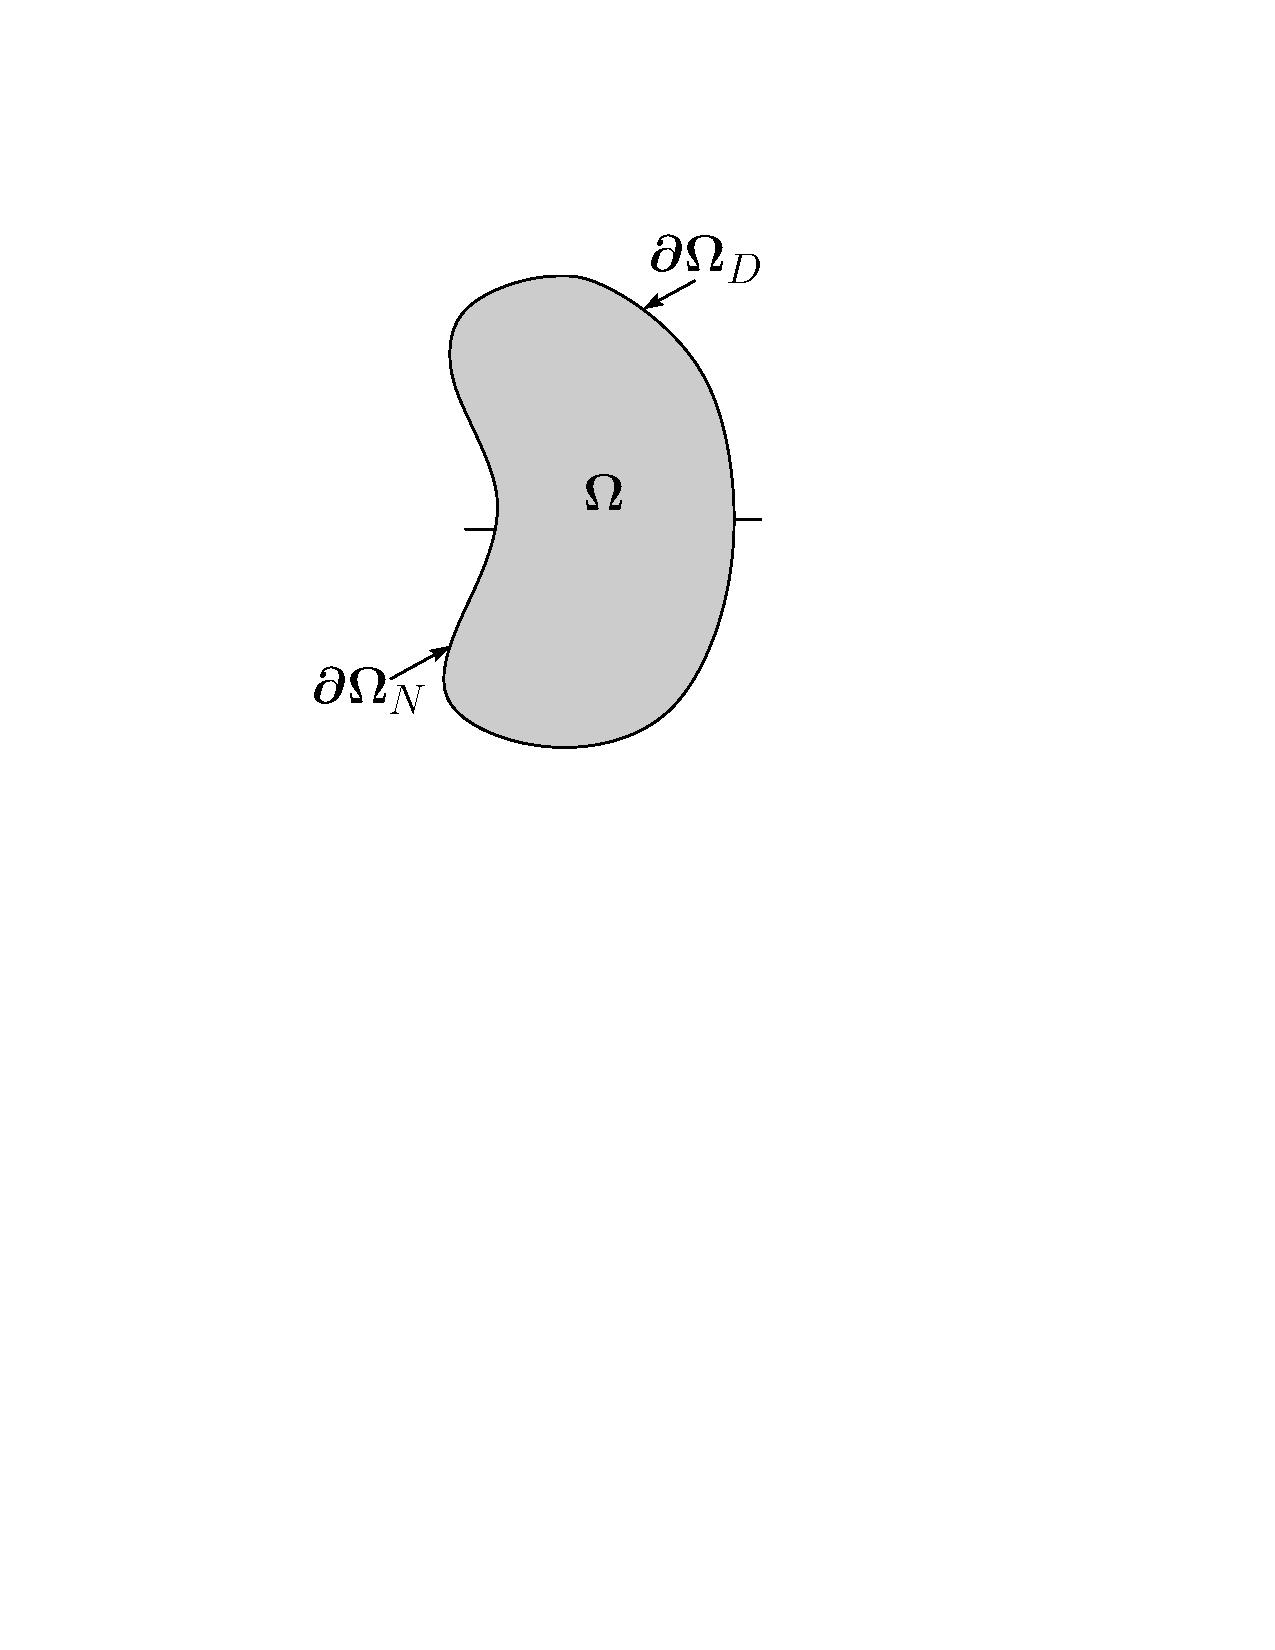
\includegraphics[viewport=140 420 400 685,clip=true,width=2in]{domain2/domain2_input}
      \end{center}
  \end{columns}
\end{frame}
